%; whizzy chapter -dvi
% -initex iniptex -latex platex -format platex -bibtex jbibtex -fmt fmt
% $B0J>e(B whizzytex $B$r;HMQ$9$k>l9g$N@_Dj!#(B
 
%     Tokyo Debian Meeting resources
%     Copyright (C) 2012 Junichi Uekawa
%     Copyright (C) 2011, 2015 Nobuhiro Iwamatsu

%     This program is free software; you can redistribute it and/or modify
%     it under the terms of the GNU General Public License as published by
%     the Free Software Foundation; either version 2 of the License, or
%     (at your option) any later version.

%     This program is distributed in the hope that it will be useful,
%     but WITHOUT ANY WARRANTY; without even the implied warranty of
%     MERCHANTABILITY or FITNESS FOR A PARTICULAR PURPOSE.  See the
%     GNU General Public License for more details.

%     You should have received a copy of the GNU General Public License
%     along with this program; if not, write to the Free Software
%     Foundation, Inc., 51 Franklin St, Fifth Floor, Boston, MA  02110-1301 USA

%  preview (shell-command (concat "evince " (replace-regexp-in-string "tex$" "pdf"(buffer-file-name)) "&"))

%%$B$3$3$+$i%X%C%@3+;O!#(B

\documentclass[mingoth,a4paper]{jsarticle}
\usepackage{monthlyreport}
% $BF|IU$rDj5A$9$k!"Kh7nJQ$o$j$^$9!#(B
\newcommand{\debmtgyear}{2016}
\newcommand{\debmtgmonth}{2}
\newcommand{\debmtgdate}{13}
% started from zero:
% (let ((year 2013) (month 7)) (+ (* (- year 2005) 12) month -1))
\newcommand{\debmtgnumber}{136}

% tikz picture $B$N0Y$N%^%/%m@_Dj(B
\usepackage[dvipdfmx]{graphicx}
\usepackage{tikz}

\begin{document}

\begin{titlepage}
\thispagestyle{empty}
% $B%?%$%H%k%Z!<%8(B:$BJT=8I,MW$JItJ,$O:G=i$N%^%/%m$KHt$P$9$3$H(B

\vspace*{-2cm}
$BBh(B\debmtgnumber{}$B2s(B $BEl5~%(%j%"(B Debian $BJY6/2q;qNA(B\\
\hspace*{-2cm}

\includegraphics{image2012-natsu/dotdeb.pdf}\\
\hfill{}\debmtgyear{}$BG/(B\debmtgmonth{}$B7n(B\debmtgdate{}$BF|(B

% $B$3$3$O%"%C%W%G!<%H$9$k$3$H(B
% $BA43QJ8;z$K$7$J$$$H%U%)%s%H$N%5%$%:$,9g$o$J$$$N$GCm0U(B
\rotatebox{10}{\fontsize{30}{30} {\gt $BFC=8(B1$B!'(BDebian$B$N>CHqEENO4IM}(B}}\\
\rotatebox{10}{\fontsize{30}{30} {\gt $BFC=8(B2$B!'(Blibhinawa$B$N(BITP/RFS}}\\
\vspace*{-2cm}
\hfill{}
\includegraphics[height=6cm]{image200502/openlogo-nd.eps}
\end{titlepage}

\newpage

\begin{minipage}[b]{0.2\hsize}
 \definecolor{titleback}{gray}{0.9}
 \colorbox{titleback}{\rotatebox{90}{\fontsize{80}{80} {\gt $B%G%S%"%sJY6/2q(B} }}
\end{minipage}
\begin{minipage}[b]{0.8\hsize}
\hrule
\vspace{2mm}
\hrule
\begin{multicols}{2}
\tableofcontents
\end{multicols}
\vspace{2mm}
\hrule
\end{minipage}

\dancersection{$B;vA02]Bj(B}{$BLnEg(B $B5.1Q(B}

$B:#2s$N;vA02]Bj$O0J2<$G$9(B:
\begin{enumerate}
\item hack time $B$K2?$r$7$^$9$+!)(B
\item $BK\JY6/2q$r$I$3$G$*CN$j$K$J$j$^$7$?$+!)(B($BG$0U2sEz(B) 
\end{enumerate}
$B$3$N2]Bj$KBP$7$FDs=P$$$?$@$$$?FbMF$O0J2<$G$9!#(B
\begin{multicols}{2}
{\small
\begin{prework}{ takaswie }
  \begin{enumerate}
  \item Q.hack time に何をしますか?\\
    A.hinawa-utils の開発。あるいはALSAの開発。\\
https://github.com/takaswie/hinawa-utils
  \item Q.本勉強会をどこでお知りになりましたか?(任意回答)\\
    A. ML
  \end{enumerate}
\end{prework}


\begin{prework}{ mkouhei }
  \begin{enumerate}
  \item Q.hack time に何をしますか?\\
    A.
    \begin{itemize}
    \item https://qa.debian.org/developer.php? login=mkouhei@palmtb.net のメンテ。
    \item パッケージ ( https://qa.debian.org/developer.php? login=mkouhei@palmtb.net ) のメンテナンス
    \item keybase.io を signing-party( caff ) のキーサーバーとして利用できないかの検証

   \end{itemize}
    \item Q.本勉強会をどこでお知りになりましたか?(任意回答)\\
    A. 常連
   \end{enumerate}
\end{prework}

\begin{prework}{ Poeto }
  \begin{enumerate}
  \item Q.hack time に何をしますか?\\
    A.「 Debian 」 の基本操作。( 数日前、インストールしたばかりなので )
  \item Q.本勉強会をどこでお知りになりましたか?(任意回答)\\
    A. Web
  \end{enumerate}
\end{prework}

\begin{prework}{ kenhys }
  \begin{enumerate}
  \item Q.hack time に何をしますか?\\
    A. 未定。
  \item Q.本勉強会をどこでお知りになりましたか?(任意回答)\\
    A. ML
  \end{enumerate}
\end{prework}

\begin{prework}{ iwamatsu }
  \begin{enumerate}
  \item Q.hack time に何をしますか?\\
    A. package メンテナンス。
  \item Q.本勉強会をどこでお知りになりましたか?(任意回答)\\
    A. ML
  \end{enumerate}
\end{prework}

\begin{prework}{ Charies }
  \begin{enumerate}
  \item Q.hack time に何をしますか?\\
    A. パッケージング。
  \end{enumerate}
\end{prework}

\begin{prework}{ dictoss }
  \begin{enumerate}
  \item Q.hack time に何をしますか?\\
    A. kfreebsd の Intel GPU ビデオドライバのデバッグ( unstable で動かなくなった)
  \item Q.本勉強会をどこでお知りになりましたか?(任意回答)\\
    A. Web
  \end{enumerate}
\end{prework}

\begin{prework}{ rosh }
  \begin{enumerate}
  \item Q.hack time に何をしますか?\\
    A. d-i に関する作業
  \item Q.本勉強会をどこでお知りになりましたか?(任意回答)\\
    A. twitter
  \end{enumerate}
\end{prework}

\begin{prework}{ wskoka }
  \begin{enumerate}
  \item Q.hack time に何をしますか?\\
    A. tilegx
  \end{enumerate}
\end{prework}

\begin{prework}{ yy\_y\_ja\_jp }
  \begin{enumerate}
  \item Q.hack time に何をしますか?\\
    A. DDTSS
  \end{enumerate}
\end{prework}

\begin{prework}{ 野島 }
  \begin{enumerate}
  \item Q.hack time に何をしますか?\\
    A. DDTSS、xmrisパッケージ化など。
  \item Q.本勉強会をどこでお知りになりましたか?(任意回答)\\
    A. 幹事なので!\\ところでセミナか、幹事やってみたい人はいつでも募集中!\\貴殿好みの勉強会にしてくれてもよくてよ!
  \end{enumerate}
\end{prework}


}
\end{multicols}

\if0
\dancersection{Debian Trivia Quiz}{$BLnEg(B $B5.1Q(B}

Debian$B$N:r:#$NOCBj$K$D$$$F$N(BQuiz$B$G$9!#(B

$B:#2s$N=PBjHO0O$O(B\url{debian-devel-announce@lists.debian.org} $B$d(B \url{debian-news@lists.debian.org}$B$KEj9F$5$l$?(B
$BFbMF$J$I$+$i$G$9!#(B

\begin{multicols}{2}
%; whizzy-master ../debianmeetingresume201311.tex
% $B0J>e$N@_Dj$r$7$F$$$k$?$a!"$3$N%U%!%$%k$G(B M-x whizzytex $B$9$k$H!"(Bwhizzytex$B$,MxMQ$G$-$^$9!#(B
%

\santaku
{2015/10/22$B$N(BDPN$B$N%a!<%k$+$iDj4|E*$K$J$,$l$F$$$?$$$/$D$+$N%H%T%C%/$,(BWeb$B$N$_$K7G<($5$l$k$h$&$K$J$j$^$7$?!#$I$3$K7G<($5$l$k!)(B}
{http://www.debian.or.jp/}
{http://www.debian.org/}
{http://bits.debian.org/}
{C}
{2015/10/22$B$N(BDPN$B$N%a!<%k$+$i!"=>MhN.$l$F$$$?(BDPN$B$N%a!<%k$N9=@.$,:~?7$5$l$^$7$?!#$3$A$i$KH<$$!"%;%-%e%j%F%#$K$D$$$F$N%"%J%&%s%9$H!"?7$7$$(BDD/DM$B$N%"%J%&%s%9$O!"(BDPN$B$N%a!<%k$K$O4^$^$l$:!"(BWeb$B%Z!<%8$K7G:\$5$l$k$N$_$H$J$j$^$7$?!#(B}

\santaku
{2015/11/7$B$K$F!"$H$"$k%$%s%9%?%s%H%a%C%;%s%8%c!<MQ%W%m%H%3%k$N%5!<%S%9$,A4(BDebian Developer$B$G;H$($k$h$&$K$J$C$?$H$N%"%J%&%s%9$,$"$j$^$7$?!#%W%m%H%3%k$NL>A0$O<!$N$I$l!)(B}
{XMPP}
{IRC}
{IP Messanger}
{A}
{XMPP$B$O%*!<%W%s$J%$%s%9%?%s%H%a%C%;%s%8%c!<MQ%W%m%H%3%k$N#1$D!#$J$*!"(BDebian$B4X78<T$NMxMQ$K$"$?$C$F>\$7$/$O!"(Bhttp://rtc.debian.org$B$r;2>H!#(B}

\santaku
{2015/10/30$B$K$F!"(BDebian$B$K$F!"(B2$B2sL\$N8xJg$,9T$o$l$?Lr$^$o$j$O<!$N$I$l!)(B}
{2016 DPN}
{technical commitee}
{2016 Debian JP$B2qD9(B}
{B}
{2$BL>$[$I!"(BDebian Developer$B$NJ}$G(Btechnical comittee$B$G3hLv$G$-$kJ}Jg=8$H$N$3$H$G$9!#8=?&(Btechnical comittee$B$N?M$i$,!"(B2015/12/31$B$GG$4|$,@Z$l$F$7$^$&$H$$$&$3$H$G!"$=$l$^$G$K8uJd<T$r5s$2$kI,MW$,$"$k$H$N$3$H$G$9!#(B}



\end{multicols}
\fi

\dancersection{$B:G6a$N(BDebian$B4XO"$N%_!<%F%#%s%0Js9p(B}{$BLnEg(B $B5.1Q(B}

\subsection{$BBh(B135$B2sEl5~%(%j%"(BDebian$BJY6/2q(B}

 $B:#2s>l=j$O(Bdots$B$5$s$r$*<Z$j$7$F$N3+:E$G$7$?!#;22C<T$O(B10$BL>$G$7$?!#(B

 $B%;%_%JFbMF$O!"(B2$BK\7z$F$G!"(B
  \begin{enumerate}
  \item $B;22C<T3'$5$s$K$h$k!V(B Debian $B:#G/$NH>G/J,$N7W2h$rN)$F$F$_$?(B $B!W(B
  \item $BLnEg$5$s$K$h$k!V(B Debian $B$G(B Linux Ftrace $B$^$o$j$r$$$8$C$F$_$?(B  $B!W(B
  \end{enumerate}
$B$G$7$?!#;D$j$N;~4V$G(Bhack time$B$r9T$$!"@.2LH/I=$r$7$^$7$?!#(B

 $B!V(BDebian $B:#G/$NH>G/J,$N7W2h$rN)$F$F$_$?!W$O!"(B2016$BG/(B6$B7nKv$^$G$N(BDebian$B%W%m%8%'%/%H$G9T$&L\I8$r=q$$$FD:$-$^$7$?!#$_$J$5$s!"$,$C$A$jL\I8$rN)$F$F$$$?$@$1$^$7$?!#$"$H$O!"<B9T$"$k$N$_$G$9$M!#(B

 $B!V(BDebian $B$G(B Linux Ftrace $B$^$o$j$r$$$8$C$F$_$?!W$O!"(Blinux kernel$B$KEk:\$5$l$F$$$k%G%P%C%0(BI/F$B$G$"$k(BFtrace$B$r(BDebian$B$GMxMQ$7$F$_$?;v$K$D$$$F8l$i$l$^$7$?!#(BDebian sid$B$KEk:\$5$l$F$$$k(Bkernel$B$,(B4.3.3$B$G$"$k$3$H$+$i!"(BUSDT$B$rMxMQ$7$F$_$?$j!"(Bkprobe$B$rMxMQ$7$?OC$r$7$^$7$?!#(BDebian$B$KEk:\$5$l$F$$$k(BFtrace$BMxMQ$N%D!<%k$G$"$k!"(Bperf-tool$B$,8E$+$C$?7o$K$D$$$F$b!"(BBUG Report\footnote{https://bugs.debian.org/813769}$B$,9T$o$l$^$7$?!#(B

  $B$^$?!"(Bhack time$B$G$9$,!"@.2L$r(Btitanpad.com$B$K5-:\$9$k;n$_$r9T$$$^$7$?!#(B
 $BI=$OA02s$N(Bhack time$BCf$N@.2L$N0lMw$H$J$j$^$9!#(B($B7I>NN,(B)

\begin{table}
\begin{center}
  \begin{tabular}{|l|p{15cm}|}
    \hline
$B;22C<T(B & $B@.2L(B \\ \hline \hline
henrich &   proposal for Debian idea
  \begin{itemize}
  \item integrate piuparts into repository pipeline
  \item replace dput $\rightarrow$ lintian + piuparts, then upload
   + prevents regression into repository
  \end{itemize} \\ \hline
kenhys & libhinawa$B$N(Bdebian/*$B$K<j$r$$$l$F$$$/$D$+(BPR$B$rEj$2$?$j!"(Bissue$B$rN)$F$?$j$7$?!#;29M!'(B
\begin{itemize}
\item \url{https://github.com/takaswie/libhinawa/pull/20}
\item \url{https://github.com/takaswie/libhinawa/pull/21}
\item \url{https://github.com/takaswie/libhinawa/pull/24}
\end{itemize}\\ \hline
tai &   \begin{itemize}
    \item $B%-!<%5%$%s$r9T$C$?!#(B caff$B$G$O$J$/<jF0$G!#(B
    Keysigning with the GNU/Linux Terminal(
    \url{http://www.phillylinux.org/keys/terminal.html})
    $B$K1h$C$F$d$C$F$_$?!#$7$+$7:G8e$N=pL>$7$?%-!<$rAw$k=j$,(BGmail$B7PM3$K$J$j=pL>!&0E9f2=$;$:$KJVAw$7$F$7$^$C$?$N$G!"(Bcaff$B$,$d$C$Q$j$$$$$N$+!&!&!&(B
  \item Debian Wiki$B$NK]Lu$7;D$7$NB3$-$r$b$/$b$/$H!#(B
  \end{itemize} \\ \hline
wskoka &   tilegx$BMQ%Q%C%1!<%8:n@.(B(10$B$3$0$i$$!#%H!<%?%k$O#1#2#0#08D$0$i$$$"$k!#!K(B\\ \hline
rosh &
  \begin{itemize}
  \item caff $B$G%-!<%5%$%s$,=PMh$?(B
  \item $BA0%^!<%8$5$l$?(BLinkstation DTS [0] $B$r%Y!<%9$K$F!"?7(BLinkstation$B%G%P%$%9(B (LS-QVL)$B$N(B DTS $B$rJL$N%f!<%6MM$,=PMh$?$H$NO"Mm$,$"$j$^$7$?!#:#=5<u$1F~$l$i$l$?(B Linkstation DTS [1] $B$K%^!<%8$r9T$$$^$7$?!#$3$l$+$i(B ARM kernel lists $B$K%"%C%W$9$kM=Dj$G$9!#(B
    \begin{enumerate}
    \item Kernel tree: arch/arm/boot/dts/kirkwood-{lswvl,lswxl}.dts
    \item \url{http://lists.infradead.org/pipermail/linux-arm-kernel/2016-January/400949.html}
    \end{enumerate}
  \end{itemize} \\ \hline
dictoss &   \begin{itemize}
  \item rasberry pi2$B$N(Bdebian jessie$B$+$i(Bbluetooth$B%F%6%j%s%0$G$-$?(B
  \item $B%-!<%5%$%s$7$^$7$?(B
  \item $BEl5~%(%j%"(BDebian$BJY6/2q$N(Bweb$B%5%$%H$r(BHTML5$BBP1~$H%9%^!<%H%U%)%sBP1~:n6H(B($B%j%]%8%H%j$N>l=j3NG'!"%=!<%9%3!<%I$rFI$s$GCf?H$H:n$j$rGD0.Cf(B)\footnote{2016$BG/(B2$B7n(B27$BF|$KL5;v%j%j!<%9$5$l!"(Btokyodebian.alioth.debian.org$B$O!"=K(B!$B%b%P%$%k%U%l%s%I%j!<$K$J$j$^$7$?(B!}
  \end{itemize} \\ \hline
$B#y(B.$B#y(B &
  \begin{itemize}
   \item $B;22C<T$H(Bkey sign$B$r9T$C$?!#(B
   \item Caff$B$G!"N/$^$C$F$$$?(B keysigning $B=hM}$N%-%e!<$r%U%i%C%7%e$G$-$?!#(B
  \end{itemize} \\ \hline
  \end{tabular}
\end{center}
\caption{hack time$B@.2L(B}
\end{table}

\begin{table}
\begin{center}
  \begin{tabular}{|l|p{15cm}|}
    \hline
$B;22C<T(B & $B@.2L(B \\ \hline \hline
takaswie & 
$B!!(BEcho Audio Corp.$B$N(BFireworks$B%G%P%$%9%b%8%e!<%k8~$1%3%^%s%I%i%$%s%D!<%k$,$@$$$?$$=q$1$?!#(B
\url{https://github.com/takaswie/hinawa-utils} \\ \hline
yy\_y\_ja\_jp & 
  \begin{itemize}
  \item uim-qt5 $B%P%0%l%]!<%H(B
  \item $B%-!<%5%$%s(B
  \item DDTSS
  \end{itemize} \\ \hline
$BLnEg(B &9$B8D$N(BDDTSS$B$N%l%S%e!<$r9T$$$^$7$?!#$J$*!"(Byorick$B$O(Btypo$B$N(B''M-x Yorick''$B$r8+Mn$H$7!"(Brequeue$B$7$^$7$?!#(B\\ \hline
  \end{tabular}
\end{center}
\caption{hack time$B@.2L(B($B$D$E$-(B)}
\end{table}

% % (query-replace-regexp "<.*?>" "")
% % (query-replace-regexp "^[	 ]\+" "")

%-------------------------------------------------------------------------------
\dancersection{Debian GNU/Linux $B>e$G$N>JEENO@_Dj$K$D$$$F(B}{$B4d>>(B}
%-------------------------------------------------------------------------------

\subsection{$B$O$8$a$K(B}

Linux $B$,%$%s%9%H!<%k$5$l$?%N!<%H(BPC$B$rMxMQ$7$F$$$k;~!"%9%Z%C%/DL$j$K%P%C%F%j$,;}$?$J$$>l9g$,B?!9$"$j$^$9!#(B
$B?tG/A0$HHf$Y$k$H(B Linux $B>e$NEE8;4IM}BP1~$b?J$s$G$$$^$9$,!"$^$@(BWindows$B$J$I$N(BOS$B$K$O$^$@$^$@5Z$P$J$$$H$3$m$,$"$j$^$9!#(B
$B$H$O8@$C$F$b%G%U%)%k%H$N>uBV$G;H$&$h$j!">/$7%Q%i%a!<%?$rA`:n$7$F$_$?$j!"4IM}MQ$N%D!<%k$r%$%s%9%H!<%k$9$k$@$1$G(B
$B%P%C%F%j$N;}$A$O$h$$$b$N$J$j$^$9!#>/$7$G$b(BDebian $B$G$N%N!<%H(BPC$B%i%$%U$r2a$4$9$?$a$K(B $B:#2s$O(B Debian GNU/Linux $B$rBj:`$K(B
$B$7$?(B $B>JEENO@_DjJ}K!$K$D$$$F@bL@$7$^$9!#(B


\subsection{$B>JEENO@_Dj$9$k$?$a$K$O(B}

$B>JEENO@_Dj$9$k$?$a$K$O$I$N$h$&$JE@$GEENO$r>CHq$7$F$$$k$N$+$r4JC1$KM}2r$7$F$*$/$3$H$,=EMW$G$9!#(B
Linux $B$N>l9g!"Bg$-$/J,$1$F0J2<$NE@$,=EMW$H$J$C$F$-$^$9!#(B

\begin{itemize}
\item CPU$B$H@)8f(B
\item $BF0:n$7$F$$$k%G%P%$%9(B
\item $BF0:n$7$F$$$k%W%m%0%i%`(B
\end{itemize}

$B$3$l$i$K$D$$$F!"(BDebian$B$G$NBP1~J}K!$K$D$$$F4JC1$K@bL@$7$^$9!#(B

\subsubsection{CPU$B$H@)8f(B}

CPU$B$G$9$,!"(BIntel$B@=(BCPU$B$N(BCPU$B>uBVA+0\$O?^(B\ref{fig:cpustate}$B$N$h$&$K$J$C$F$*$j!"(BCPU$B2TF/>uBV$H(B
$B%9%j!<%W>uBV$N@Z$jBX$($,IQHK$K9T$o$l$F$$$^$9!#(BCPU$B$K$O%9%F!<%H!J(BC$B%9%F!<%H!K$H$$$&>uBV$,$"$j!"(B
$B$3$N>uBV$K$h$C$F>CHqEENO$,0[$J$j!"(BCPU$B$NI|5";~4V$bJQ$o$C$F$-$^$9!#:G?7$N(BCPU$B$G$O$b$C$H:Y$+$$%9%F!<%H$,Ds6!(B
$B$5$l$k$h$&$K$J$C$F$$$^$9!#$3$l$i$r@)8f$7$F$$$k$N$,(BACPI$B$H$J$j$^$9!#(B

\begin{figure}[H]
\begin{center}
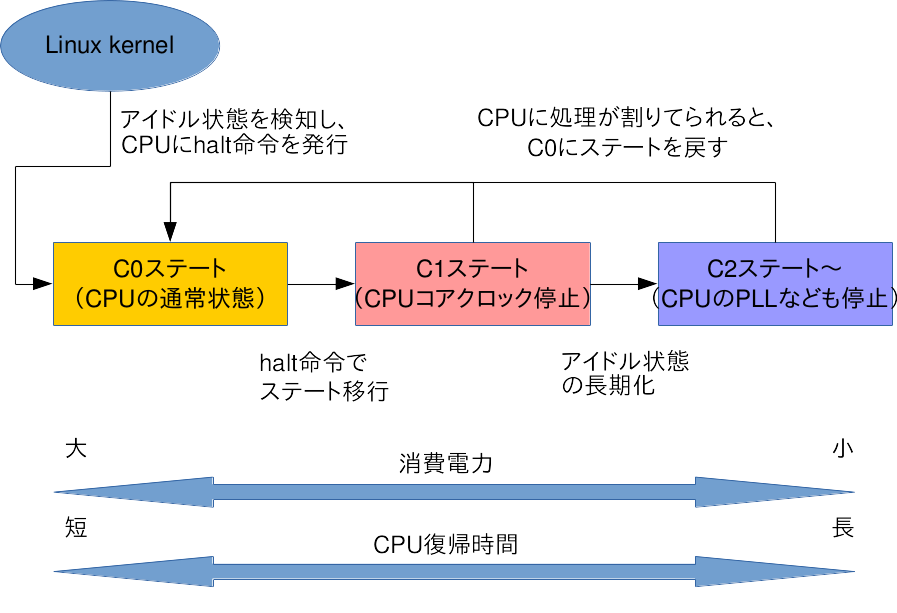
\includegraphics[width=0.5\hsize]{image201602/cpustate.png}
\end{center}
\label{fig:cpustate}
\caption{CPU$B>uBVA+0\4J0W?^(B} 
\end{figure}

$B<B:]$N(BCPU$B$O(BC$B%9%F!<%H$@$1$G$O$J$/!"(BCPU$B$NEE05$d%/%m%C%/?t$J$I$b4XO"$7$F$-$^$9!#(B
Linux $B$N>l9g$O(BCPU$B<~GH?t%9%1!<%j%s%05!G=$r;H$&$3$H$G!"(BOS$B$,<+F0E*$K@)8f$G$-$k$h$&$K$J$C$F$$$^$9!#(B
$B$3$l$O(B Linux $B%+!<%M%k$N(B cpufreq $B$K$h$C$F<BAu$5$l$F$$$^$9!#(B
$B8=:_$N(B cpufreq $B$K@_Dj$5$l$F$$$kFbMF$r3NG'$9$k$K$O(B cpufrequtils $B%Q%C%1!<%8$GDs6!$5$l$F$$$k(B
cpufreq-info$B!J(B\ref{fig:cpufreq-info}$B!K(B $B%3%^%s%I$r;H$$$^$9!#(B

\begin{figure}[htbp]
\begin{commandline}
$ cpufreq-info
cpufrequtils 008: cpufreq-info (C) Dominik Brodowski 2004-2009
Report errors and bugs to cpufreq@vger.kernel.org, please.
analyzing CPU 0:
  driver: intel_pstate
  CPUs which run at the same hardware frequency: 0
  CPUs which need to have their frequency coordinated by software: 0
  maximum transition latency: 0.97 ms.
  hardware limits: 800 MHz - 2.90 GHz
  available cpufreq governors: performance, powersave
  current policy: frequency should be within 800 MHz and 2.90 GHz.
                  The governor "powersave" may decide which speed to use
                  within this range.
  current CPU frequency is 1.90 GHz.
....
\end{commandline}

\caption{cpufreq-info $B<B9T7k2L(B}
\label{fig:cpufreq-info}
\end{figure}

$B$$$/$D$+9`L\$,$"$j$^$9$,!"=EMW$H$J$k$N$O(B $B!V(Bavailable cpufreq governors$B!W$H(B
$B!V(Bcurrent policy$B!W$G$9!#(B
available cpufreq governors $B$O(B CPU$B$ND4@02DG=$JB.EYD4@0L>!J%,%P%J!<!K$G$"$j!"(B
$B0J2<$N$b$N$,MQ0U$5$l$F$$$^$9!#(B

\begin{table}[htb]
\begin{center}
\begin{tabular}{l|l}
$B%,%P%J!<(B & $BFbMF(B \\
ondemand &	CPU$BIi2Y$,Bg$-$$!"$^$?$O>.$5$$;~$K(BCPU$B%/%m%C%/$rBg$-$/$K@Z$jBX$($k(B \\
conservative &	CPU$BIi2Y$,Bg$-$$!"$^$?$O>.$5$$;~$K(BCPU$B%/%m%C%/$r=y!9$K@Z$jBX$($k(B \\
performance &	$B:GBg<~GH?t$G(BCPU$B$rF0:n$5$;$k(B \\
powersave &	$B:G>.<~GH?t$G(BCPU$B$rF0:n$5$;$k(B \\
userspace &	$B%f!<%6!<$,;XDj$7$?<~GH?t$G(BCPU$B$rF0:n$5$;$k(B \\
\end{tabular}
\caption{$B;XDj$G$-$k%,%P%J!<(B}
\label{tab:governors}
\end{center}
\end{table}

$B$3$l$i$O<B:]$K$O@_Dj$G$-$kCM%+!<%M%k$d4D6-$K$h$C$F0[$J$kE@$KCm0U$,I,MW$G$9!#(B
$B!V(Bcurrent policy$B!W$O8=:_@_Dj$5$l$F$$$k%,%P%J!<$,I=<($5$l$^$9!#(B

$B$3$N0J>e$+$i!">e5-$N7k2L$G$O(B

\begin{itemize}
\item CPU$B$,(B800MHz$B$+$i(B2.90GHz$B$^$G$r%5%]!<%H$7$F$$$k(B
\item powersave governor $B$GF0:n$7$F$$$k(B
\item $B:GBgCM$H:G>.CM$N%]%j%7!<@_Dj$K$h$j!"(B800MHz$B$+$i(B2.90GHz$B$N4V$GJQF0$5$;$F$$$k(B
\end{itemize}

$B$H$$$&$3$H$,$o$+$j$^$9!#(B

$B$3$l$i$r@_Dj$9$k$K$O(B sysfs $B7PM3$GA`:n$9$k$+!"(Bcpufrequtils $B$K4^$^$l$k(B
cpufreq-set $B%3%^%s%I$r;H$$$^$9!#(B

\begin{itemize}
\item $B%,%P%J!<$r@_Dj$9$k(B
  \begin{commandline}
   $ sudo cpufreq-set -c CPU$BHV9f(B -g $B%,%P%J!<L>(B
   $B$^$?$O(B
   $ sudo sh -c "echo $B%,%P%J!<L>(B > /sys/devices/system/cpu/cpuCPU$BHV9f(B/cpufreq/scaling_governor"
  \end{commandline}

\item $B:G>.%/%m%C%/$r@_Dj$9$k(B
  \begin{commandline}
   $ sudo cpufreq-set -c CPU$BHV9f(B -d $B%/%m%C%/CM(B
   $B$^$?$O(B
   $ sudo sh -c "echo $B%/%m%C%/CM(B > /sys/devices/system/cpu/cpuCPU$BHV9f(B/cpufreq/scaling_min_freq"
  \end{commandline}

\item $B:GBg%/%m%C%/$r@_Dj$9$k(B
  \begin{commandline}
   $ sudo cpufreq-set -c CPU$BHV9f(B -u $B%/%m%C%/CM(B
   $B$^$?$O(B
   $ sudo sh -c "echo $B%/%m%C%/CM(B > /sys/devices/system/cpu/cpuCPU$BHV9f(B/cpufreq/scaling_max_freq"
  \end{commandline}

\item $B8=:_$N%/%m%C%/$r@_Dj$9$k(B
  \begin{commandline}
   $ sudo cpufreq-set -c CPU$BHV9f(B -f $B%/%m%C%/CM(B
   $B$^$?$O(B
   $ sudo sh -c "echo $B%/%m%C%/CM(B > /sys/devices/system/cpu/cpuCPU$BHV9f(B/cpufreq/scaling_cur_freq"
  \end{commandline}

\end{itemize}

$B>e5-$N$h$&$K$7$F(BCPU$B%/%m%C%/$r@)8f$9$k$3$H$K$h$j!"4D6-$K$h$C$FL5BL$J$/(BCPU$B$rMxMQ$G$-$k$h$&$K$J$j$^$9!#(B
$B@_Dj$7$?CM$O:F5/F0$9$k$H>C$($k$N$G!"(B/etc/sysfs.conf $B$K@_Dj$7$F$*$/$+!"(Bcpufreq $B$r@_Dj$9$k%G!<%b%s(B cpufreqd
$B$r;H$&$H$h$$$G$7$g$&!#(B

\subsubsection{$BF0:n$7$F$$$k%G%P%$%9$N@_Dj(B}

$B;H$C$F$$$k8D!9$N%G%P%$%9$N@_Dj$b=EMW$H$J$j$^$9!#Nc$($PL5@~(BLAN$B$d(BBluetooth$B$r;H$o$J$$$N$KM-8z$K$7$F$$$k$H(B
$B$=$l$@$1$GEENO$r>CHq$7$F$7$^$$$^$9!#$h$C$F;HMQ$9$k4D6-$K1~$8$F$3$l$i$r@)8f$9$kI,MW$,=P$F$-$^$9!#(B

$B$3$3$G$O$h$/MxMQ$5$l$k%G%P%$%9$KBP$9$k@)8fJ}K!$K$D$$$F@bL@$7$^$9!#(B

\begin{itemize}

\item $B%i%C%W%H%C%W%b!<%I(B

Linux $B$N>l9g$O%+!<%M%k$N%b!<%I$H$7$F!"%i%C%W%H%C%W%b!<%I$,@_Dj$G$-$k$h$&$K$J$C$F$$$^$9!#(B
$B$3$l$O0J2<$N$h$&$K$7$F@_Dj$7$^$9!#(B

\begin{commandline}
$ sudo sh -c "echo 5 > /proc/sys/vm/laptop_mode"
\end{commandline}

$B$"$H(BNMI $B$N(Bwatchdog$B!J(Bnmi\_watchdog$B!K(B $B$bL58z2=$7$F$*$-$^$9!#$3$l$O$3$l$O%+!<%M%k%O%s%0%"%C%W$rDj4|E*$K%A%'%C%/$9$k5!9=(B
$B$r%3%s%H%m!<%k$9$k%U%i%0$G$9!#(B

\begin{commandline}
$ sudo sh -c "echo 0 > /proc/sys/kernel/nmi_watchdog"
\end{commandline}

\item USB

USB $B$O(B /sys/bus/usb/devices/ $B0J2<$KBP$7$F@_Dj$r9T$$$^$9!#(B
$BNc$($P!"(B/sys/bus/usb/devices/usb1 $B$KBP$7$F(B $BEE8;6!5k$r@Z$j$?$$>l9g$O(B /sys/bus/usb/devices/usb1/power/control
$B$r(Boff $B$K@_Dj$7$^$9!#<+F0E*$K%5%9%Z%s%I$5$;$?$$>l9g$K$O(B 
/sys/bus/usb/devices/usb1/power/autosuspend $B$KBP$7$F(B 1 $B$r@_Dj$7$^$9!#(B

\begin{commandline}
$ sudo sh -c "echo off > /sys/bus/usb/devices/usb1/power/control"
$ sudo sh -c "echo auto > /sys/bus/usb/devices/usb1/power/autosuspend"
\end{commandline}

$B@_Dj$r5/F0;~$KE,MQ$7$?$$>l9g$O!":F5/F0;~$K=i4|2=$5$l$F$7$^$&;v$H%G%P%$%9$N(BUSB$B0LCV$,JQ$o$k;v$,(B
$B$"$j$^$9$N$G!"(B udev $B$N(B rules $B%U%!%$%k$r;H$C$F@_Dj$9$k$N$,$h$$$G$7$g$&!#(B

\begin{commandline}
$ cat /etc/udev/rules.d/70-my-usb-power.rules
ACTION=="add", SUBSYSTEM=="usb", ATTRS{idVendor}=="0x046d", ATTR{idProduct}=="0x08cb", TEST=="power/control", ATTR{power/control}="off"
\end{commandline}

$BCm0U$7$J$1$l$P$$$1$J$$E@$H$7$F$O(BUSB$B$r$J$s$G$b@_Dj$7$F$7$^$&$H%-!<%\!<%I$,F0:n$7$J$/$J$k2DG=@-$b$"$k$?$a!"(B
$B%Y%s%@!<(BID$B!"%G%P%$%9(BID$B$J$I$r3NG'$7$?>e$G@_Dj$7$^$7$g$&!#(B

\item $BL5@~(BLAN

$BL5@~(BLAN$B$O(B iw $B%Q%C%1!<%8$K4^$^$l$k(B iw $B%3%^%s%I$r;H$C$F@_Dj$7$^$9!#(B
$BL5@~(BLAN$B$,(Bwlan0$B$N>l9g$O(B $B0J2<$N$h$&$K@_Dj$9$k$3$H$K$h$C$F@)8f$G$-$^$9!#(B

\begin{commandline}
$ sudo iw dev wlan0 set power_save on
\end{commandline}

$B$3$l$b(Budev $B$N(B rules $B%U%!%$%k$r;H$C$F@_Dj$9$k$HNI$$$G$9!#(B

\begin{commandline}
$ cat /etc/udev/rules.d/70-my-wifi-power.rules
ACTION=="add", SUBSYSTEM=="net", KERNEL=="wlan*", RUN+="/usr/bin/iw dev %k set power_save on"
\end{commandline}

\item $B%5%&%s%I(B

$B%5%&%s%I$N>l9g$b(B sysfs $B7PM3$G@_Dj$7$^$9!#%I%i%$%P$K$h$C$F@_Dj=PMh$J$$>l9g$,$"$j$^$9$,!"(BINTEL $B$N%5%&%s%I(B
$B%3%s%H%m!<%i$N>l9g$O!"(Bpower\_save $B$,$"$k$N$G!"$3$l$r(B1$B$K@_Dj$9$k$3$H$K$h$C$F%Q%o!<%;!<%V%b!<%I$K@_Dj$G$-$^$9!#(B

\begin{commandline}
$ sudo sh -c "echo 1 > /sys/module/snd_hda_intel/parameters/power_save"
\end{commandline}

\item PCI/PCI-Express

PCI/PCI-Express $B$N>JEENO$K@_Dj$9$k$K$O(B power/control $B$r(B auto $B$K@_Dj$7$^$9!#(B
$B$3$N>l9g$b(B sysfs $B7PM3$G@_Dj$7$^$9!#(BPCI$B$b(BUSB$B$HF1MM$K@_Dj@h$,$I$N$h$&$J%G%P%$%9(B
$B$J$N$+3NG'$7$F$+$i@_Dj$9$k$h$&$K$7$^$7$g$&!#(B

\begin{commandline}
$ sudo sh -c "echo auto > /sys/bus/pci/devices/0000:00:00.0/power/control"
\end{commandline}

\end{itemize}

\subsubsection{$BF0:n$7$F$$$k%W%m%0%i%`$K$D$$$F(B}

$BF0:n$7$F$$$k%W%m%0%i%`$O(Btop$B%3%^%s%I$J$N$G$6$C$/$j$H$7$?(BCPU$B@jM-N($r3NG'$G$-$^$9$,!"<B:]$K(B
$B$I$l$0$i$$$NIQEY$G;H$o$l$F$F$$$k$N$+$o$+$j$^$;$s!#%"%$%I%k>uBV$G$"$k$K$b$+$+$o$i$:!"(BCPU$B3d$j9~$_$,B?$$(B
$B%W%m%0%i%`!&%W%m%;%9$,>JEENO$N8z2L$,F@$K$/$$$b$N$H$J$j$^$9$N$G!"$3$N$h$&$J%W%m%0%i%`!&%W%m%;%9$r(B
$BD4$Y$kI,MW$,$"$j$^$9!#$3$l$i$rD4$Y$k$K$O2<5-$G@bL@$9$k(B PowerTop $B$r;H$&$H$h$&$G$7$g$&!#(B

\subsection{$B>JEENO@_Dj$9$k$?$a$N%D!<%k(B}

$B@h$G$OD9!9$H=q$-$^$7$?$,!"CN<1$,$J$$%f!<%6$,>e5-$r0l$D$E$D$d$C$F$$$/$N$OHs>o$KBgJQ$G$9!#(B
Linux $B$G$O@lLg$NCN<1$,$J$/$H$b;H$C$F$$$k%^%7%s$r>JEENO>uBV$K@_Dj$G$-$k%D!<%k$,$$$/$D$+(B
$B=`Hw$5$l$F$$$^$9!#0J2<$G$O$=$l$i$N;H$$J}$K$D$$$F>R2p$7$^$9!#(B

\subsubsection{PowerTOP}

PowerTOP $B$O(BIntel$B$,3+H/$7$F$$$k%=%U%H%&%'%"$G!"%+!<%M%k!"%O!<%I%&%'%"!"%f!<%6%i%s%I$G@)8f2DG=$J>JEENO9`L\$r(B
$BM-8z$K$9$k%D!<%k$G$9!#%W%m%;%9$r4F;k$7$F!"(BCPU$BIi2Y$d%G%P%$%9%I%i%$%P$N;HMQ>u67$N%l%]!<%H$+$i%W%m%;%9$NA`:n(B
$B$r9T$&;v$,$G$-$^$9!#(B

\begin{enumerate}

\item $B%$%s%9%H!<%k(B

PowerTOP $B$O(BDebian $B$G$bDs6!$5$l$F$*$j!"(Bapt $B$G%$%s%9%H!<%k$G$-$^$9!#(B
\begin{commandline}
% sudo apt-get install powertop	
\end{commandline}

\item $B5/F0(B

$B5/F0$9$k$H?^(B\ref{fig:powertop0}$B$N$h$&$J2hLL$,I=<($5$l$^$9!#(B
$B!V(BThe battery reports a discharge rate ...$B!W(B $B$K8=:_$N>CHqEENO$,(B
$BI=<($5$l!"8=:_F0:n$7$F$$$k%W%m%;%9$H;HMQ>u67$,$o$+$j$^$9!#(B
$BI.<T$N4D6-$G!"2?$b@_Dj$7$J$$>l9g$O(B 13W$B$N$h$&$G$9!#(B

\begin{figure}[H]
\begin{center}
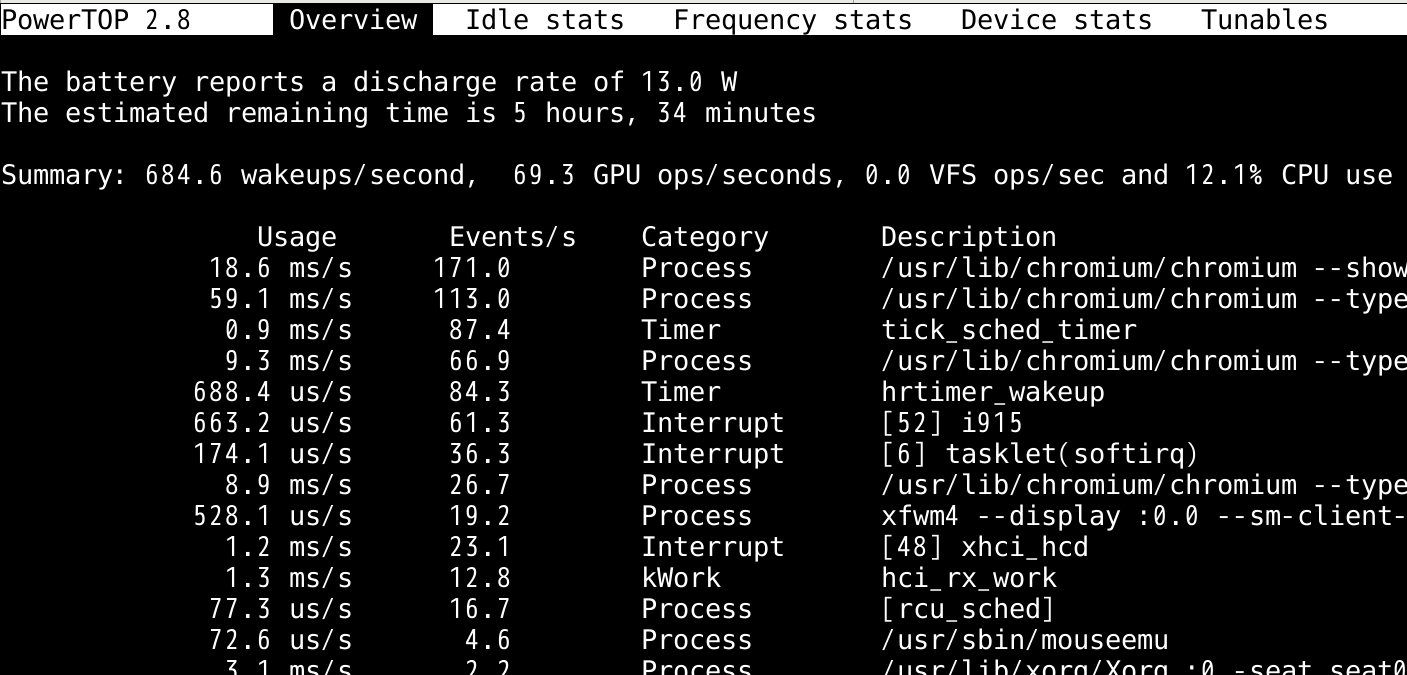
\includegraphics[width=0.5\hsize]{image201602/powertop_00.png}
\end{center}
\label{fig:powertop0}
\caption{PowerTOP$B5/F02hLL(B} 
\end{figure}

Tunables $B%?%V$rA*Br$9$k$HD4@02DG=$J%7%9%F%`$N@_Dj$,I=<($5$l$^$9!#(B
Bad$B$,>JEENO$KM-8z$J9`L\$K$b$+$+$o$i$:L58z$J@_Dj!"(B
Good $B$,4{$KM-8z$K$J$C$F$$$k@_Dj$H$J$C$F$$$^$9!#(B

\begin{figure}[H]
\begin{center}
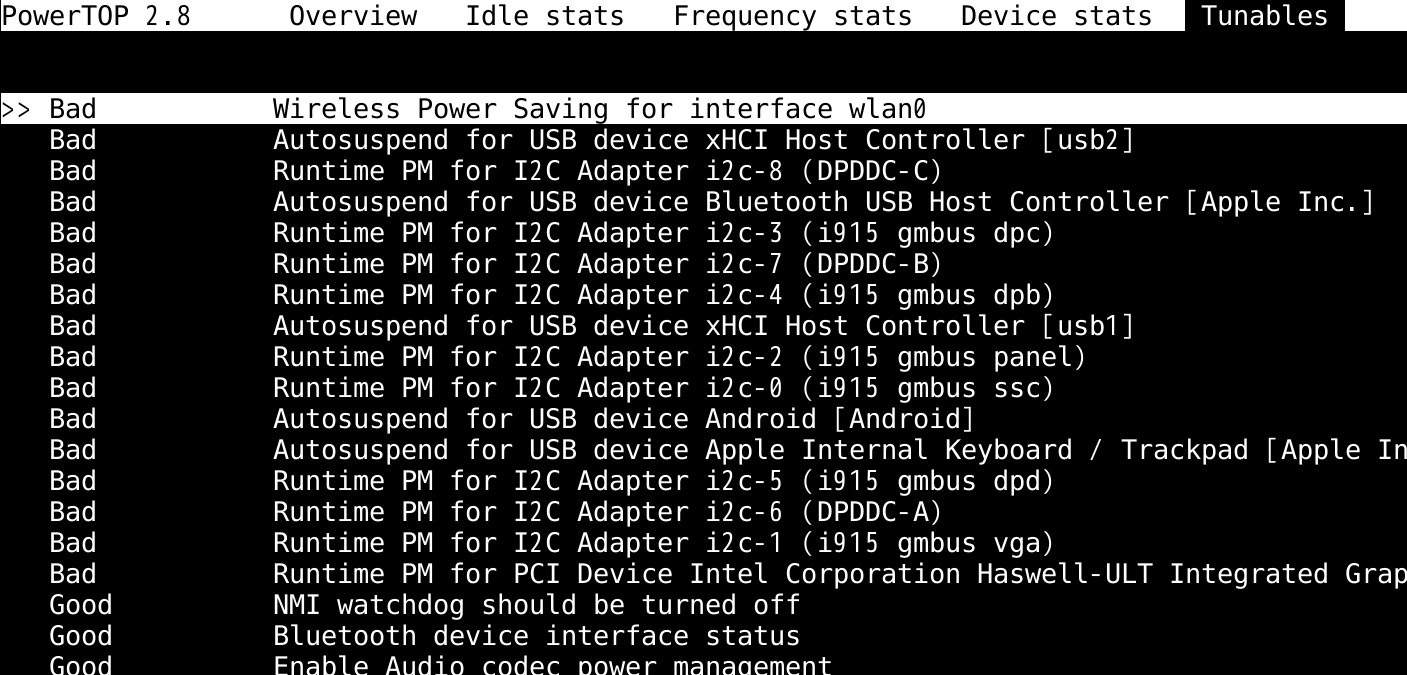
\includegraphics[width=0.5\hsize]{image201602/powertop_01.png}
\end{center}
\label{fig:powertop1}
\caption{Tunables$B2hLL(B} 
\end{figure}

$B$3$N>uBV$G$O$^$@%7%9%F%`$K:GE,2=$5$l$?@_Dj$K$J$C$F$$$J$$$?$a!"0lEY=*N;$7!"(B
$B%-%c%j%V%l!<%7%g%s$r9T$$$^$9!#(B

\item $B%-%c%j%V%l!<%7%g%s(B

$B@_Dj$9$k(BPC$B$N>uBV$r<hF@$9$k$?$a$K%-%c%j%V%l!<%7%g%s$r9T$$$^$9!#(B
$B<B9T$9$k$H%G%P%$%9$J$I$+$i;HMQ>u67$rFI$_<h$j!"%^%7%s$KBP$7$FE,@Z$J@_Dj$r(B
$B9T$$$^$9!#(B
$B%N!<%H(BPC$B$N>l9g$O$$$-$J$j%b%K%?!<$N%P%C%/%i%$%H$,>C$($k$N$GCm0U$7$^$7$g$&!#(B

\begin{commandline}
$ sudo powertop --calibrate
\end{commandline}

$B%-%c%j%V%l!<%7%g%s$,=*$o$k$H!"(B\texttt{/var/cache/powertop/saved\_parameters.powertop}
$B0J2<$K%G!<%?$,J]B8$5$l$^$9!#<!2s$N(BPowerTOP$B5/F0;~$+$i$O%-%c%j%V%l!<%7%g%s%G!<%?$r85$K(B
$B>JEENO$K$5$l$?4D6-$G5/F0$7$^$9!#(B

\item $B%-%c%j%V%l!<%7%g%s8e(B

$B%-%c%j%V%l!<%7%g%s8e$K5/F0$9$k$H!"(B
$B!V(BThe battery reports a discharge rate ...$B!W(B $B$N9`L\$KI=<($5$l$k>CHqEENOCM$,JQ$o$j!"%7%9%F%`(B
$BA4BN$G>JEENO$G2TF/$7$F$$$k$3$H$,3NG'$G$-$k$G$7$g$&!#(B

\item PowerTOP $B$N5/F0;~M-8z2=(B

PowerTOP $B$O5/F0$9$k$HJ]B8$5$l$F$$$k@_Dj$r85$K>JEENO>uBV$K$7$F$/$l$^$9$,!"(BPC$B$rN)$A>e$2$k$?$S$K(B
PowerTOP$B<+BN$rN)$A>e$2$kI,MW$,$"$j$^$9!#(B

$B5/F0;~$K<+F0E*$K(BPowerTOP $B$rN)$A>e$2$k$h$&$K$9$k$K$O!"0J2<$N$h$&$K(B systemd $B$N(B $B%f%K%C%H%U%!%$%k(B
$B$rMQ0U$7!"M-8z$K$7$F$*$-$^$9!#(B

\begin{commandline}
$ cat /etc/systemd/system/powertop.service

[Unit]
Description=PowerTOP

[Service]
Type=oneshot
ExecStart=/usr/bin/powertop
Environment="TERM=xterm"

[Install]
WantedBy=multi-user.target
\end{commandline}

\begin{commandline}
$ sudo systemctl enable powertop
\end{commandline}

\end{enumerate}

\subsubsection{TLP $B$r;H$C$?@_Dj(B}

PowerTOP $B$NB>$K(BTLP$B$H$$$&%D!<%k$b$"$j$^$9!#$3$l$O(B PowerTOP$B$N$h$&$K>\:Y$J%l%]!<%H$O(B
$B=P$7$F$/$l$^$;$s$,!"(BAC$B@\B3;~$J$I$N>u67$K1~$8$?%9%/%j%W%H$,=`Hw$5$l$F$*$j!"%$%s%9%H!<%k(B
$B$9$k$@$1$G$"$kDxEY>JEENO@_Dj$r9T$C$F$/$l$kJXMx$J%D!<%k$G$9!#(B
$B$b$A$m$s!"(BDebian $B$G$O%Q%C%1!<%82=$5$l$F$*$j!"(Bapt $B$G%$%s%9%H!<%k$G$-$^$9!#(B

\begin{commandline}
$ sudo apt-get install tlp
\end{commandline}

$BL5@~(BLAN$B$N@_DjEy$K(B NetworkManager $B$r;H$C$F$$$k$J$i(B tlp-rdw $B%Q%C%1!<%8$b%$%s%9%H!<%k$7$F$*$/$H(B
$BL5@~(BLAN$B!"(BBluetooth$B4XO"$N@_Dj$b9T$C$F$/$l$^$9!#(B
$B%G%U%)%k%H$N@_Dj$O(B /etc/default/tlp $B$K$"$j!"$3$N%U%!%$%k$rJQ99$7$F4D6-$K9g$o$;$?>JEENO@_Dj$r(B
$B9T$$$^$9!J?^(B\ref{fig:TLP}$B!K!#@_Dj$O$h$/;H$o$l$k9`L\$7$+$J$/!";H$C$F$$$k4D6-$N@_Dj$,$J$$>l9g$b$"$j$^$9!#$3$N$h$&$J>l9g$O(B
T$B<+J,$G@_Dj$rDI2C$9$k$+!"@h$K@bL@$7$?$h$&$K(Bsysfs / procfs $B7PM3(B
$B$N@_Dj$rJLES9T$&I,MW$,$"$j$^$9!#(B


\begin{figure}[H]
\begin{center}
\begin{commandline}
# Set to 0 to disable, 1 to enable TLP.
TLP_ENABLE=1

# Operation mode when no power supply can be detected: AC, BAT
# Concerns some desktop and embedded hardware only.
TLP_DEFAULT_MODE=AC

# Seconds laptop mode has to wait after the disk goes idle before doing a sync.
# Non-zero value enables, zero disables laptop mode.
DISK_IDLE_SECS_ON_AC=0
DISK_IDLE_SECS_ON_BAT=2

# Dirty page values (timeouts in secs).
MAX_LOST_WORK_SECS_ON_AC=15
MAX_LOST_WORK_SECS_ON_BAT=60
...
\end{commandline}
\end{center}
\label{fig:TLP}
\caption{/etc/default/tlp $BNc(B} 
\end{figure}

TLP $B$O(B systemd $B$d$=$NB>(Binit$BMQ$N5/F0%U%!%$%k$,MQ0U$5$l$F$$$k$N$G(BPC$B5/F0;~$K@_Dj$,H?1G$5$l$k$N$b(B
$BNI$$E@$G$9!#(B

\subsubsection{$B>JEENO@_Dj8e(B}
$B?^(B\ref{fig:powertop2}$B$,>JEENO@_Dj$7$?8e$K(B PowerTOP $B$G>CHqEENO$r3NG'$7$?FbMF$G$9!#(B
$B>CHqEENO$,(B13W $B$+$i(B 11W $B$K2<$,$C$F$$$k$3$H$,$o$+$j$^$9!#$^$?(BPC$B2TF/;~4V$b(B5$B;~4VH>$+$i(B6$B;~4V(B50$BJ,$K(B
$B?-$S$F$$$k$3$H$,$o$+$j$^$9!#(B

\begin{figure}[H]
\begin{center}
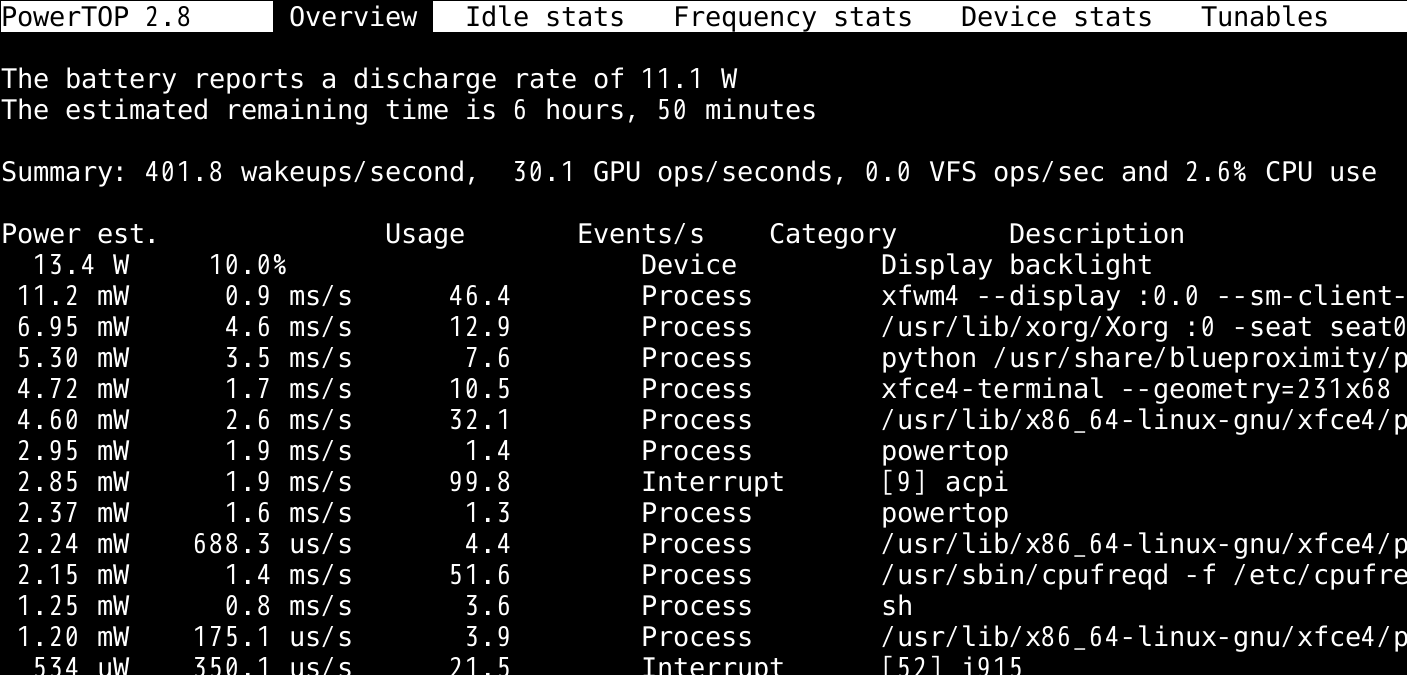
\includegraphics[width=0.5\hsize]{image201602/powertop_02.png}
\end{center}
\label{fig:powertop2}
\caption{$B>JEENO@_Dj8e(B} 
\end{figure}

\subsection{$B$^$H$a(B}

Debian $B$G$N>JEENO@_Dj$K$D$$$F@bL@$7$^$7$?!#(B
$B8=:_$N>uBV$r$H$j$"$($:3NG'$9$k$K$O(B cpufreq-info $B$r;H$$!"%+!<%M%k$N@_Dj$d%I%i%$%P$N@_Dj$O(B
sysfs $B$d(B proc fs $B7PM3$G@_Dj$7$^$9!#%W%m%0%i%`$d%W%m%;%9$N>\:Y$J>uBV$N3NG'$9$k$K$O(B PowerTOP
$B$r;H$$$^$9!#>JEENO@_Dj$G$-$k9`L\$b$o$+$j!"%f!<%6%$%s%?!<%U%'%$%9$+$i3F<o@_Dj$,$G$-$k$h$&$K$J$C$F$$$^$9!#(B
$B$^$?:FN)$A>e$2$9$k$H>JEENO@_Dj$r:F@_Dj$9$kI,MW$,$"$j$^$9$N$G!"(Bsysytem$BMQ$N(Bservice
$B%U%!%$%k$rJLESMQ0U$9$k$J$I$NBP:v$,I,MW$G$9!#(B
$B:Y$+$$@_Dj$r9T$o$J$/$F$b!"$H$j$"$($:>JEENO@_Dj$r9T$$$?$$>l9g$O(BTLP$B$r;H$&$N$,$h$$$G$7$g$&!#$?$@A4$F$N(B
PC$B$r%5%]!<%H$7$F$$$k$o$1$G$O$"$j$^$;$s$N$G!"4D6-$K9g$o$;$F%W%m%0%i%`$r=$@5$9$k$J$j$NBP1~$,I,MW$H$J$j$^$9!#(B


%-------------------------------------------------------------------------------
\dancersection{libhinawa $B$H$$$&%i%$%V%i%j$r(B Debian $B%W%m%8%'%/%H$K(B ITP/RFS $B$7$?OC(B}{takaswie}
%-------------------------------------------------------------------------------

\subsection{$B$O$8$a$K(B}

%-------------------------------------------------------------------------------
\dancersection{$B2q>l$G$NL5@~(BLAN$B$N$D$J$.J}(B}{$BLnEg(B $B5.1Q(B,Roger}
%-------------------------------------------------------------------------------
 \subsection{$B$O$8$a$K(B}

$B!!:#2s2q>lB&$K$OL5@~(BLAN$B7PM3$N%0%m!<%P%k2s@~$,MQ0U$5$l$F$$$^$9!#(B

$B!!0J2<$K(BDebian$B%^%7%s$G$N@\B3J}K!$r5-:\$7$^$9!#(B

 $B$^$?!"<+J,$N4D6-$G$O0c$&$d$jJ}$G$D$J$,$C$?$H$$$&J}$O!"LnEg$^$G(B
$B65$($F2<$5$$!#$3$A$i$G$b%N%&%O%&$H$7$FN/$a$F$$$/M=Dj$G$9!#(B

 \subsection{wpasupplicant$B5Z$S(B/etc/network/interfaces$B$rMxMQ$N>l9g(B}

 $B$b$C$H$bNI$$%^%K%e%"%k$O!"(B/usr/share/doc/wpasupplicant/README.Debian.gz
$B$H$J$j$^$9!#:$$C$?>l9g$O$3$A$i$b9g$o$;$F$4;2>H2<$5$$!#(B

$B!!0J2<$K(B/etc/network/interfaces$B$NDj5A$K$D$$$F2q>l$NNc$r5-:\$7$^$9!#(B

\begin{commandline}
$ sudo vi /etc/network/interfaces
-----$B0J2<$N%(%s%H%j$,$J$1$l$PDI5-$3$3$+$i(B----------
iface wlan0_debian inet dhcp
     wpa-conf /etc/wpa_supplicant/wpa_supplicant_debian.conf
-----$B0J2<$N%(%s%H%j$,$J$1$l$PDI5-$3$3$^$G(B----------
$ sudo vi /etc/wpa_supplicant/wpa_supplicant_debian.conf
-----$B0J2<$N%(%s%H%j$rDI5-$3$3$+$i(B----------
network={
     ssid=<<$B2q>l$N(BSSID>>
     psk=<<$B2q>l$N%Q%9%o!<%I(B>>
     scan_ssid=1
}
-----$B0J2<$N%(%s%H%j$rDI5-$3$3$^$G(B----------
$ sudo chmod 600 /etc/wpa_supplicant/wpa_supplicant_debian.conf
$ sudo ifup wlan0=wlan0_debian
\end{commandline}
%$

 $B$^$?!"%O%^$C$F$7$^$C$?;~$N%G%P%C%0J}K!$O!"(B
/usr/share/doc/wpasupplicant/README.Debian.gz$BCf$N(B''4. Trubleshooting''$B$N>O$,JXMx$G$9!#(B

 \subsection{$B$=$NB>$NL5@~(BLAN$BMQ%Q%C%1!<%8$rMxMQ$N>l9g(B}

$B!!$9$_$^$;$s!"<+J,$,>pJs$r;}$?$J$$$?$a!"8=>l$G65$($F2<$5$$!#(B

\cleartooddpage

\vspace*{15cm}
\hrule
\vspace{2mm}

\includegraphics[width=2cm]{image200502/openlogo-nd.eps}
\noindent \Large \bf Debian $BJY6/2q;qNA(B\\
\noindent \normalfont \debmtgyear{}$BG/(B\debmtgmonth{}$B7n(B\debmtgdate{}$BF|(B \hspace{5mm}  $B=iHGBh(B1$B:~H/9T(B\\
\noindent \normalfont $BEl5~%(%j%"(B Debian $BJY6/2q(B $B!JJT=8!&0u:~!&H/9T!K(B\\
\hrule

\end{document}
